\section{稳定性与收敛}
\label{sec:pdenum-stability}

前面三种方法都用到了同一个模式：差分方程上是$\lVert\bm{A}_h^{-1}\rVert_\infty\leq1/8$，Galerkin方法上是强制常数，扩散方程上是放大因子不超过$1$。这里把这些词的含义固定下来，并说明线性问题和非线性守恒问题为什么不能共用一条判据。

\paragraph{三个概念}
比较不同网格上的解，先要选定一族离散范数。常用的有
\[
 \lVert\bm{v}\rVert_{\infty}=\max_j\lvert v_j\rvert,\qquad
 \lVert\bm{v}\rVert_{1,h}=h\sum_j\lvert v_j\rvert,\qquad
 \lVert\bm{v}\rVert_{2,h}=\Bigl(h\sum_j\lvert v_j\rvert^2\Bigr)^{1/2}.
\]
下面的概念都依赖于范数的选取，同一个格式可以在一种范数下稳定，在另一种范数下不稳定。

对线性单步格式$\bm{U}^{(k+1)}=\bm{B}_\tau\bm{U}^{(k)}$，$h$随$\tau$按固定的关系变化，三个概念的含义如下。

\begin{definition}[一致性、稳定性与收敛]
 \label{def:pdenum-consistency-stability}
 设真解充分光滑，局部误差$\bm{\eta}^{(k)}$由下式定义：
 \begin{equation}
  \bm{R}_hu(t_{k+1})=\bm{B}_\tau\bm{R}_hu(t_k)+\tau\,\bm{\eta}^{(k)} .
  \label{eq:pdenum-local-error}
 \end{equation}
 若$\max_k\lVert\bm{\eta}^{(k)}\rVert\to0$，称格式\term{一致}（consistent）。若存在$\tau_0,C_T$，使
 \begin{equation}
  \lVert\bm{B}_\tau^k\rVert\leq C_T\qquad\text{对所有}\ 0<\tau\leq\tau_0,\ k\tau\leq T,
  \label{eq:pdenum-stable}
 \end{equation}
 称格式\term{稳定}（stable）。若$k\tau\to t$时$\bm{U}^{(k)}$与$\bm{R}_hu(t)$的差趋于零，称格式收敛（convergent）。
\end{definition}

稳定性是对离散算子幂的一致界，常数$C_T$允许依赖$T$，它只描述有限时间。

\subsection{线性格式}
\label{sec:pdenum-linear}

\paragraph{一致性加稳定性}
由式~\eqref{eq:pdenum-local-error}减去格式本身，$\bm{e}^{(k)}=\bm{R}_hu(t_k)-\bm{U}^{(k)}$满足
\[
 \bm{e}^{(k+1)}=\bm{B}_\tau\bm{e}^{(k)}+\tau\bm{\eta}^{(k)} .
\]
递推展开，得到
\begin{equation}
 \bm{e}^{(k)}=\bm{B}_\tau^k\bm{e}^{(0)}+\tau\sum_{l=0}^{k-1}\bm{B}_\tau^{k-1-l}\bm{\eta}^{(l)} .
 \label{eq:pdenum-error-duhamel}
\end{equation}
用稳定性估计每个幂，得到
\begin{equation}
 \lVert\bm{e}^{(k)}\rVert\leq C_T\Bigl(\lVert\bm{e}^{(0)}\rVert+T\max_l\lVert\bm{\eta}^{(l)}\rVert\Bigr).
 \label{eq:pdenum-lax-bound}
\end{equation}
一致性保证右端趋于零，这就是收敛，收敛阶就是局部误差的阶。

反过来，收敛能否推出稳定？在恰当的框架下回答是肯定的。为了让所有网格落在同一个空间里，这里把格式看成一个Banach空间上的算子族，网格函数延拓成分片常数函数后就落入这个框架。

\begin{theorem}[Lax等价定理]
 \label{thm:pdenum-lax}
 设$X$是Banach空间，$S(t)$是适定线性初值问题的解算子，在$[0,T]$上一致有界且强连续。$B_\tau$是$X$上的有界线性算子，在稠密子集$D\subset X$上一致，即对$u_0\in D$，
 \begin{equation}
  \frac{1}{\tau}\sup_{k\tau\leq T}\bigl\lVert\bigl(B_\tau S(k\tau)-S((k+1)\tau)\bigr)u_0\bigr\rVert\to0 .
  \label{eq:pdenum-lax-consistent}
 \end{equation}
 则格式稳定，当且仅当对每个$u_0\in X$，只要$\tau\to0$且$k\tau\to t\in[0,T]$，就有$B_\tau^ku_0\to S(t)u_0$。
\end{theorem}

\begin{proof}
 先证稳定推出收敛。对$u_0\in D$，望远镜求和给出
 \[
  B_\tau^ku_0-S(k\tau)u_0=\sum_{l=0}^{k-1}B_\tau^{k-1-l}\bigl(B_\tau S(l\tau)-S((l+1)\tau)\bigr)u_0 .
 \]
 由稳定性和条件~\eqref{eq:pdenum-lax-consistent}，右端的范数不超过$C_Tk\tau$乘以一个趋于零的量。

 对一般的$u_0\in X$，用$D$中的元素逼近它。稳定性控制$B_\tau^k$作用在差上的量，$S(k\tau)$的一致有界性控制另一边，所以$B_\tau^ku_0-S(k\tau)u_0\to0$。再由强连续性，$S(k\tau)u_0\to S(t)u_0$。

 再证收敛推出稳定。假设格式不稳定，则存在$\tau_n\to0$和$k_n$，$k_n\tau_n\leq T$，使$\lVert B_{\tau_n}^{k_n}\rVert\to\infty$。取子序列使$k_n\tau_n\to t$。对每个$u_0\in X$，收敛性说明序列$B_{\tau_n}^{k_n}u_0$收敛，因而有界。由一致有界原理，$\sup_n\lVert B_{\tau_n}^{k_n}\rVert<\infty$，矛盾。
\end{proof}

定理的前提不可省略：问题必须线性且适定，格式必须线性，收敛要对$X$中每一个初值成立。

\paragraph{扩散格式的稳定估计}
显式Euler方法的稳定性可以用两种范数验证。在$\lVert\cdot\rVert_{2,h}$下，$\bm{I}-\tau\bm{A}_h$对称，特征值是$1-\tau\lambda_m$，所以范数不超过$1$的条件正是式~\eqref{eq:pdenum-ftcs-stability}，此时$C_T=1$。

在$\lVert\cdot\rVert_\infty$下，$r\leq1/2$时，式~\eqref{eq:pdenum-ftcs-component}可以写成
\[
 U_j^{(k+1)}=(1-2r)U_j^{(k)}+rU_{j-1}^{(k)}+rU_{j+1}^{(k)},
\]
三个系数非负且和为$1$，新值是旧值的凸组合，于是
\[
 \lVert\bm{U}^{(k+1)}\rVert_\infty\leq\lVert\bm{U}^{(k)}\rVert_\infty .
\]
这是热的抹平在离散层面上的体现。

\paragraph{Fourier稳定性分析}
规则网格、常系数、周期边界（或全直线）的情形，离散Fourier变换把格式对角化。把模式$U_j=\mathrm{e}^{\mathrm{i}j\xi}$代入格式，$\xi\in[-\pi,\pi]$，每步乘上一个放大因子$g(\xi)$。由Parseval恒等式，
\begin{equation}
 \lVert\bm{B}_\tau^k\rVert_{2,h}=\max_\xi\lvert g(\xi)\rvert^k .
 \label{eq:pdenum-von-neumann}
\end{equation}
稳定的充要条件是存在$C$，使$\lvert g(\xi)\rvert\leq1+C\tau$对所有$\xi$成立。

扩散格式~\eqref{eq:pdenum-ftcs-component}的放大因子是
\[
 g(\xi)=1+r(\mathrm{e}^{-\mathrm{i}\xi}-2+\mathrm{e}^{\mathrm{i}\xi})=1-4r\sin^2\frac{\xi}{2} .
\]
它在$\xi=\pi$时取到最小值$1-4r$，$\lvert g\rvert\leq1$的条件是$r\leq1/2$，与上面的结论一致。

迎风格式~\eqref{eq:pdenum-upwind}的放大因子$g(\xi)=1-\mu(1-\mathrm{e}^{-\mathrm{i}\xi})$在复平面上是以$1-\mu$为心、半径$\mu$的圆，并且
\begin{equation}
 \lvert g(\xi)\rvert^2=1-4\mu(1-\mu)\sin^2\frac{\xi}{2} .
 \label{eq:pdenum-upwind-factor}
\end{equation}
所以$0\leq\mu\leq1$时稳定。中心差分通量的放大因子是$g(\xi)=1-\mathrm{i}\mu\sin\xi$，$\lvert g\rvert^2=1+\mu^2\sin^2\xi$，对固定的$\mu>0$都大于$1$（$\sin\xi=0$处除外），这就是图~\ref{fig:pdenum-upwind-smear}(b)中振荡的来源。图~\ref{fig:pdenum-fourier-factors}把这三种情形画在复平面上，轨迹跑出单位圆的部分就是被放大的模式。

\begin{BookInlineFigure}
 \centering
 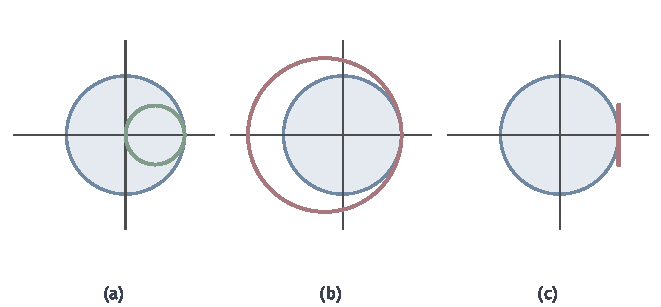
\includegraphics[width=112mm]{figures/06-differential-equations/02-partial-differential-equations/matplotlib/pdenum-fourier-factors/figure.pdf}
 \caption{输运格式的放大因子$g(\xi)$在复平面上的轨迹，浅蓝圆盘是$\lvert g\rvert\leq1$。(a)迎风格式$\mu=0.5$（绿），轨迹在圆盘内。(b)迎风格式$\mu=1.3$（红），最大模$1.6$，大部分在圆盘外。(c)中心差分$\mu=0.5$（红），轨迹是一段竖直线段，只在切点处不在圆外，最大模约为$1.118$。}
 \label{fig:pdenum-fourier-factors}
\end{BookInlineFigure}

\paragraph{边界闭合要单独检查}
Fourier分析的前提是周期边界或全直线，真实问题的边界不属于这个情形。边界的处理可能破坏内部的稳定性。

对$(0,1)$上的热方程，左端加上散热边界$\partial_xu(0,t)=\beta u(0,t)$，$\beta>0$，这个条件在物理上是耗散的。用虚拟节点$U_{-1}$和中心差分$(U_1-U_{-1})/(2h)=\beta U_0$消去虚拟节点，边界节点的更新是
\begin{equation}
 U_0^{(k+1)}=\bigl(1-2r(1+\beta h)\bigr)U_0^{(k)}+2rU_1^{(k)} .
 \label{eq:pdenum-robin-closure}
\end{equation}

系数非负的条件是$r\leq1/(2+2\beta h)$，比内部条件$r\leq1/2$更严。取$h=1/20$，$\beta=20$，$r=0.45$，内部的Fourier条件满足，边界节点的系数却是$-0.8$，迭代矩阵的谱半径是$1.173$，结果见图~\ref{fig:pdenum-boundary-closure}。

\begin{BookInlineFigure}
 \centering
 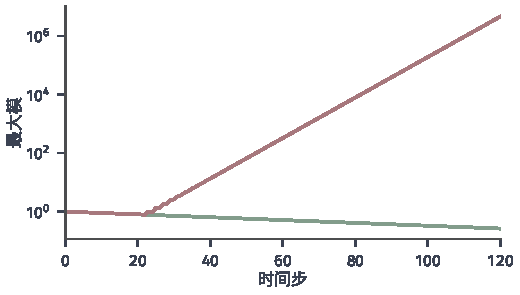
\includegraphics[width=88mm]{figures/06-differential-equations/02-partial-differential-equations/matplotlib/pdenum-boundary-closure/figure.pdf}
 \caption{显式格式解热方程的最大模随时间步的变化，$h=1/20$，$r=0.45$，右端$u=0$。绿线是左端Dirichlet条件，谱半径$0.990$，解衰减。红线是左端的散热条件~\eqref{eq:pdenum-robin-closure}，$\beta=20$，谱半径$1.173$，内部完全相同的格式发生指数增长。}
 \label{fig:pdenum-boundary-closure}
\end{BookInlineFigure}

反过来，只看矩阵的特征值也可能误判。对迎风格式取$\mu=1.5$，入流边界取零，矩阵是下双对角矩阵，特征值全是$-0.5$，谱半径小于$1$。可是这个矩阵远非正规，$N=20$时$\lVert\bm{B}^k\rVert_2$在$k=1,5,10,20$上依次约为$2.0$、$31.5$、$982$、$8.0\times10^5$，暂态增长足以毁掉计算。

\subsection{CFL条件}
\label{sec:pdenum-cfl}

上面得到的$\mu\leq1$有一个不依赖放大因子的解释：数值解必须能够看到它应该看到的初值。

\paragraph{依赖区域的比较}
对$\partial_tu+a\partial_xu=0$，$a>0$，点$(x_j,t_k)$的解等于初值在特征线足点$x_j-at_k$处的值（第~\ref{chap:transport-equations}章）。迎风格式每走一步只向左多看一个单元，所以$U_j^{(k)}$依赖的初值位于$[x_j-kh,x_j]$。

足点的距离是$at_k=\mu kh$，要落在这个区间内，就要$\mu\leq1$。图~\ref{fig:pdenum-cfl-domains}是两种情形的对比。

\begin{BookInlineFigure}
 \centering
 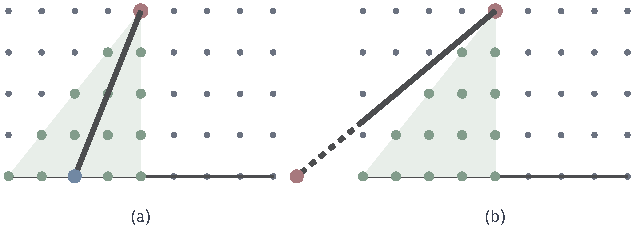
\includegraphics[width=107mm]{figures/06-differential-equations/02-partial-differential-equations/tikz/pdenum-cfl-domains/figure.pdf}
 \caption{迎风格式的依赖区域，顶部红点是要计算的值，绿点和浅绿三角形是它依赖的网格点，粗线是过红点的特征线。(a)$\mu=0.5$，足点（蓝）在依赖区域内。(b)$\mu=1.5$，特征线从依赖区域左侧穿出，足点（红）落在格式看不到的地方。}
 \label{fig:pdenum-cfl-domains}
\end{BookInlineFigure}

\begin{theorem}[CFL条件的必要性]
 \label{thm:pdenum-cfl}
 考虑$\partial_tu+a\partial_xu=0$的显式格式，步长比$\mu=a\tau/h$固定，单步模板向上游最多延伸$m$个单元。若$\mu>m$，则格式不可能对所有连续的初值收敛。
\end{theorem}

\begin{proof}
 固定$(x,t)$，$t>0$。$k\tau=t$时，$U_j^{(k)}$只依赖距$x_j$不超过$mkh$的上游初值，而
 \[
  mkh=m\,t\,\frac{h}{\tau}=\frac{m}{\mu}\,at<at .
 \]
 所以足点$x-at$与依赖区域之间有一段固定的距离。

 取一个在依赖区域内为零、在足点处非零的连续初值$u_0$。数值解在所有网格上都恒为零，而真解是$u_0(x-at)\ne0$，所以不收敛。
\end{proof}

这个条件称为\term{CFL条件}（Courant--Friedrichs--Lewy condition）。定理说的是必要性，反过来不成立：中心差分格式在$\mu\leq1$时满足CFL条件，但放大因子大于$1$，并不稳定。依赖区域够大只说明格式有可能拿到正确信息，这些信息是否被正确使用，还要看更新系数和边界处理。

$\mu=1.5$时，迎风格式对初值$(0,1,0,0)$走一步是$(0,-0.5,1.5,0)$，第二步是$(0,0.25,-1.5,2.25)$，最大模每步放大$1.5$倍。

用同样的比较看其他情形。隐式格式的依赖区域是整个网格，CFL条件自动满足，但这不等于大步长下精度也好。Burgers方程的特征速度依赖解，条件成为$\lambda\max\lvert u\rvert\leq1$，与式~\eqref{eq:pdenum-monotone-cfl}吻合。

热方程的显式格式的依赖区域宽度是$2kh=2t\,h/\tau$，连续问题的依赖区域是整条线，要填满它只需$h/\tau\to\infty$。$\tau\sim h^2$自然满足这一点，可见$r\leq1/2$这个限制并不是CFL条件，它更严格，来自稳定性。

\subsection{非线性守恒格式}
\label{sec:pdenum-nonlinear}

Lax等价定理依赖线性：误差传播写成了$\bm{B}_\tau$的幂。非线性守恒律的解甚至会在有限时间产生间断，因此要换一条路线，把“极限是什么”和“是否收敛”分开回答。

\begin{theorem}[Lax--Wendroff定理]
 \label{thm:pdenum-lax-wendroff}
 设$\widehat{F}$相容且局部Lipschitz，$\lambda=\tau/h$固定，$U^{(h)}(x,t)$是式~\eqref{eq:pdenum-conservative}的解构成的分片常数函数，初值取$u_0\in L^\infty(\mathbb{R})$的单元平均。若$h\to0$时$U^{(h)}$一致有界，且在$L^1_{\mathrm{loc}}$中收敛到$u$，则$u$是式~\eqref{eq:pdenum-conservation-law}的弱解，即对每个$\phi\in C_c^\infty(\mathbb{R}\times[0,T))$，
 \begin{equation}
  \int_0^T\!\!\int_{\mathbb{R}}\bigl(u\,\partial_t\phi+F(u)\,\partial_x\phi\bigr)\,\mathrm{d}x\,\mathrm{d}t+\int_{\mathbb{R}}u_0\,\phi(x,0)\,\mathrm{d}x=0 .
  \label{eq:pdenum-lw-limit}
 \end{equation}
\end{theorem}

\begin{proof}
 记$\phi_j^{(k)}=\phi(x_j,t_k)$。把式~\eqref{eq:pdenum-conservative}乘以$h\phi_j^{(k)}$，对$j,k$求和，再在时间和空间上分别作Abel求和，把差分转到$\phi$上。$\phi$有紧支集，没有边界项，得到
 \[
  \begin{aligned}
  &h\sum_jU_j^{(0)}\phi_j^{(0)}
  +h\tau\sum_{k\geq1}\sum_jU_j^{(k)}\frac{\phi_j^{(k)}-\phi_j^{(k-1)}}{\tau}\\
  &\qquad+h\tau\sum_{k\geq0}\sum_j\widehat{F}_{j+1/2}^{(k)}\frac{\phi_{j+1}^{(k)}-\phi_j^{(k)}}{h}=0 .
  \end{aligned}
 \]

 第一项趋于$\int u_0\phi(x,0)\,\mathrm{d}x$，因为$U_j^{(0)}$是单元平均。第二项中差商一致趋于$\partial_t\phi$，又有$U^{(h)}\to u$，所以它趋于$\iint u\,\partial_t\phi$。

 第三项要用相容性。把$\widehat{F}_{j+1/2}^{(k)}$换成$F(U_j^{(k)})=\widehat{F}(U_j^{(k)},U_j^{(k)})$，由Lipschitz性质，代价不超过常数乘以
 \[
  h\tau\sum_{k,j}\lvert U_{j+1}^{(k)}-U_j^{(k)}\rvert ,
 \]
 求和只在$\phi$的支集附近进行。这个量是$U^{(h)}$平移$h$前后之差的$L^1$范数，由$U^{(h)}$在$L^1_{\mathrm{loc}}$中收敛和平移的连续性，它趋于零。余下的部分趋于$\iint F(u)\,\partial_x\phi$，这里用到$F$的局部Lipschitz性和一致有界性。
\end{proof}

定理的假设里已经包含了收敛，它只回答极限是什么，也没有说是哪一个弱解。图~\ref{fig:pdenum-entropy-fix}(b)的Roe型通量相容又守恒，数值解收敛到的是膨胀激波这个错误的弱解。

要得到熵解，需要把定理~\ref{thm:pdenum-discrete-entropy}的不等式传到极限。对$\phi\geq0$作与上面相同的Abel求和，不等式保持方向，极限给出
\begin{equation}
 \begin{gathered}
 \iint\bigl(\lvert u-c\rvert\,\partial_t\phi+\mathrm{sgn}(u-c)(F(u)-F(c))\,\partial_x\phi\bigr)\,\mathrm{d}x\,\mathrm{d}t\\
 +\int\lvert u_0-c\rvert\,\phi(x,0)\,\mathrm{d}x\geq0 .
 \end{gathered}
 \label{eq:pdenum-entropy-limit}
\end{equation}
这对每个常数$c$成立，正是第~\ref{chap:scalar-conservation-laws}章的Kružkov熵条件，满足它的解是唯一的。

余下的问题是收敛本身。单调格式的解不超出初值的上下界，这是单调性和常数状态不变的直接推论。全变差也不增加，由Helly选择定理可得$L^1_{\mathrm{loc}}$中收敛的子序列；全变差不增的证明需要Crandall--Tartar引理，篇幅较长，读者可查阅守恒律数值方法的专著。子序列的极限都是唯一的熵解，所以整个序列收敛。

表~\ref{tab:pdenum-linear-nonlinear}对比两种论证。三件事分别对应三个不同的工具，少了哪一个都不够。

\begin{BookInlineTable}
 \centering
 \caption{线性问题与非线性守恒律的收敛论证。}
 \label{tab:pdenum-linear-nonlinear}
 \begin{tabular}{p{20mm}p{34mm}p{40mm}}
  \toprule
  要回答的问题 & 线性格式 & 非线性守恒格式\\
  \midrule
  是否收敛 & 一致性加稳定性（Lax等价） & 有界性加全变差控制给出紧性\\
  极限是什么 & 自动是原问题的解 & 守恒且相容（Lax--Wendroff）\\
  选出哪个解 & 解唯一，无须选择 & 离散熵不等式（单调格式）\\
  误差的范数 & $\lVert\cdot\rVert_{2,h}$等 & 通常是$L^1_{\mathrm{loc}}$，间断处不用最大模\\
  \bottomrule
 \end{tabular}
\end{BookInlineTable}

收敛速度也不同。图~\ref{fig:pdenum-godunov-shock}的激波问题在$T=0.8$时，单元数取$40$、$80$、$160$、$320$、$640$，$L^1$误差依次为
\[
 0.0300,\quad 0.0144,\quad 0.0079,\quad 0.0035,\quad 0.0019,
\]
观测阶略有起伏，整体接近$1$。
